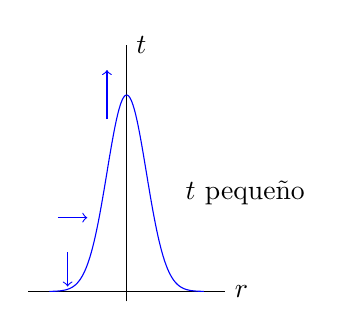
\begin{tikzpicture}[scale=1.25]

\draw (-1, 0) -- (1, 0) node[right] { $r$};
\draw (0, -0.1) -- (0, 2.5) node[right] {$t$};

\def\sigma{0.2};
\def\mu{0};

\draw[samples=300, domain=-pi/4:pi/4, blue] plot ({\x}, {( 1/sqrt( 2* \sigma^2 * pi)) * e^(-((\x - \mu)^ 2 ) / (2*\sigma^ 2)) });

\draw[->, blue]  (-0.6, 0.4) -- (-0.6, 0.05);
\draw[->, blue]  (-0.7, 0.75) -- (-0.4, 0.75);
\draw[->, blue]  (-0.2, 1.75) -- (-0.2, 2.25);
\node[right] at (0.5, 1) {$t$ pequeño};

\end{tikzpicture}